\documentclass[11pt]{article}
\usepackage[utf8]{inputenc}

% General-use Packages
\usepackage{amsmath}
\usepackage{amssymb}
\usepackage{graphicx}
\usepackage[margin=1truein]{geometry}
\usepackage{xcolor}
\usepackage{tikz}
\usepackage{pgfplots}
\usepackage{enumerate}
\usepackage{tcolorbox}

%Document-specific Packages%

\usepackage{sectsty}
\usepackage{scrextend}
\usepackage{mathtools}
\usepackage{etoolbox} % used for the \isempty command
\usepackage{xifthen} % used for \ifthenelse

% Meta
\title{MAT137 Test 3 Notebook}
\author{Ian Huang}
\date{\today}

% Number set macros
\def\Z{{\mathbb Z}}
\def\Q{{\mathbb Q}}
\def\R{{\mathbb R}}
\def\C{{\mathbb C}}
\def\N{{\mathbb N}}

% For graphing
\pgfplotsset{soldot/.style={only marks,mark=*},
             holdot/.style={fill=white,only marks,mark=*},
             compat=1.12}

% Theorem and Definition boxes
\definecolor{_orange}{HTML}{ff9e54}
\definecolor{_orange2}{HTML}{fff5ed}
\definecolor{_blue}{HTML}{519aed}
\definecolor{_blue2}{HTML}{e8f3ff}
\definecolor{_grey}{HTML}{3b3b3b}

\newenvironment{definition}[1][]{\begin{tcolorbox}[colframe=_orange,colback=_orange2,title=Definition. \ifthenelse{\isempty{#1}}{}{(#1)}
]}{\end{tcolorbox}}
\newenvironment{theorem}[1][]{\begin{tcolorbox}[colframe=_blue,colback=_blue2,title=Theorem. \ifthenelse{\isempty{#1}}{}{(#1)}
]}{\end{tcolorbox}}

% "Solution" box
\newenvironment{solution}{\begin{tcolorbox}[colframe=_grey,colback=white,arc=0pt,outer arc=0pt]}{\end{tcolorbox}}

% Colored "TRUE" and "FALSE" elements
\newcommand{\true}{\textbf{\textcolor[HTML]{26de57}{TRUE}}}
\newcommand{\false}{\textbf{\textcolor[HTML]{f54242}{FALSE}}}

% Definitions for ceiling and floor symbols
\DeclarePairedDelimiter\ceil{\lceil}{\rceil}
\DeclarePairedDelimiter\floor{\lfloor}{\rfloor}

% Definitions for norm symbols
\newcommand\norm[1]{\left\lVert#1\right\rVert}

% Utility Macros
\newcommand{\hr}{\noindent\makebox[\linewidth]{\rule{\textwidth}{0.4pt}}\par\vspace{0.1in}}
\newcommand{\emptyline}[0]{\\\hfill$~$\\}
\newenvironment{proof}{\par\textit{\textbf{Proof.}}}{\hfill$\blacksquare$}


% Formatting settings
\sectionfont{\LARGE}
\subsectionfont{\Large}
\subsubsectionfont{\large}
\paragraphfont{\large}

% Disable paragraph indents
\setlength{\parindent}{0pt}

% Configure section numbering
\setcounter{secnumdepth}{2}

\begin{document}

\maketitle
\tableofcontents
\newpage
\section{Unit 6: Applications of Limits and Derivatives}
\section{Unit 7: The Definition of Integral}
\subsection{Sigma Notation}
The notation for sums uses the capital Greek letter $\Sigma$
$$
    \sum_{i=1}^n a_i=a_1+a_2+\dots+a_n
$$
From a programming perspective, the above statement is equivalent to the following code:
\begin{verbatim}
    sum = 0;
    
    for (n=1; n<=i; n++) {
        sum += a[i];
    }
\end{verbatim}
\subsubsection{Useful Formulas}

\begin{alignat*}{3}
     & \sum_{i=0}^n i   &  & =\frac{n(n+1)}{2}      &  & =1+2+\dots+n       \\
     & \sum_{i=0}^n i^2 &  & =\frac{n(n+1)(n+2)}{6} &  & =1^2+2^2+\dots+n^2 \\
     & \sum_{i=0}^n i^3 &  & =\frac{n^2(n+1)^2}{4}  &  & =1^3+2^3+\dots+n^3
\end{alignat*}
\subsubsection{Properties}
Let $i_0,n\in\Z$. \emptyline
\textbf{Distributive Property}
$$
    \sum_{i=i_0}^n(c\cdot a_i)=c\left(\sum_{i=i_0}^n a_i\right)
$$
\textbf{Associative/Commutative Property}
$$
    \sum_{i=i_0}^n(a_i+b_i)=\sum_{i=i_0}^na_i+\sum_{i=i_0}^nb_i
$$
\subsection{Supremum and Infimum}
\subsubsection{Definitions}
\begin{definition}
    Let $A\subseteq\R$. Let $c\in\R$.
    \begin{enumerate}
        \item $c$ is an \textbf{upper bound} of $A$ when
              $$\forall x\in A,~x\leq c$$
        \item $c$ is the \textbf{least upper bound} or \textbf{supremum} of $A$ when
              \begin{enumerate}
                  \item $c$ is an upper bound of $A$
                  \item If $b\in\R$ is an upper bound of $A$, then $c\leq b$. In other words,
                        $$
                            \forall b\in\R, x\in A,~x\leq b\implies c\leq b
                        $$
              \end{enumerate}
              We denote this value ``$\sup A$''.
        \item If $\sup A\in A$, then $\sup A=\max A$.
        \item $A$ is \textbf{bounded above} when $A$ has at least one upper bound.
    \end{enumerate}
\end{definition}
This definition can be extended to the definition of infimum. $c$ is a \textit{lower bound} of $A$ when $\forall x\in A,~x\geq c$; $c$ is the \textit{infimum} of $A$ when it is the \textit{greatest upper bound} and so on.
\begin{definition}[Supremum of a Function]
    The \textbf{supremum of a function $f$ on a domain $I$}, denoted {\small$\displaystyle\sup_{x\in I}f(x)$}, is equal to
    $$
        \sup\{f(x):x\in I\}
    $$
\end{definition}
\subsubsection{Theorems}
\begin{theorem}[Lowest Upper Bound Principle]
    Let $A\subseteq\R$. \\
    IF
    \begin{enumerate}
        \item $A$ is bounded above
        \item $A$ is not empty
    \end{enumerate}
    THEN $A$ has a least upper bound.
\end{theorem}
\begin{theorem}
    Let $f$ be a function defined on a domain $I\neq \emptyset$.\\If $f$ is bounded above on $I$, then $f$ has a supremum on $I$.
\end{theorem}
Note the similarity between the above theorem and the Extreme Value Theorem that states that for a continuous function $f$ defined on $[a,b]$, there exists both a maximum and minimum on $[a,b]$.
\subsubsection{Supremum and the Empty Set}
The following are true about the empty set, $\emptyset$:
\begin{enumerate}
    \item \textbf{Every real number is an upper bound of $\emptyset$.} \\
          Remember that for some statement
          $$\forall n\in S,~C(n)$$
          If $S$ is empty, then the condition $C(n)$ is irrelevant; the statement is always (vacuously) true.
    \item \textbf{$\emptyset$ does not have a supremum.} \\
          From statement (1), we see that there is no least upper bound for $\emptyset$.
    \item \textbf{$\emptyset$ has no maximum.} \\
          The definition of maximum uses an existential quantifier; there are no elements of $\emptyset$.
    \item \textbf{$\emptyset$ is bounded above.}
\end{enumerate}
\subsubsection{Examples}
Let $A,B\subseteq\R$. Which of the following are true?
\begin{enumerate}
    \item If $B\subseteq A$ and $A$ is bounded above, then $B$ is bounded above.
          \begin{solution}
              This statement is \true.
              \begin{proof}
                  We have that $A$ is bounded above; therefore, there exists some upper bound $x$, for which all elements of $A$ are less than or equal to $x$. Because, $B$ is a subset of $A$, all elements of $B$ are also less than or equal to $x$.
              \end{proof}
          \end{solution}
    \item If $B\subseteq A$ and $B$ is bounded above, then $A$ is bounded above.
          \begin{solution}
              This statement is \false. Take $A=\R$ and $B=[0,1]$ as a counterexample.
          \end{solution}
    \item If $B\subseteq A$ and $A$ is bounded above, then $\sup B\leq \sup A$.
          \begin{solution}
              This statement is \true, assuming both $A$ and $B$ are non-empty. Otherwise, take $B=\emptyset$ and $\sup B$ does not exist.
              \begin{proof}
                  From statement (1), we have that $B$ is also bounded above; then, by the lowest upper bound principle, we have both $A$ and $B$ have a supremum.
                  \\ Imagine that $\sup B>\sup A$; there must be some value $x\in B$ such that $x>\sup A$. Because $B\subseteq A$, $x$ must be simultaneously an element of $A$ and also greater than every element in $A$, which is impossible. Therefore, $\sup B \leq \sup A$.
              \end{proof}
          \end{solution}
    \item If $A$ and $B$ are bounded above, then $\sup(A\cap B)=\min\{\sup A,\sup B\}$.
          \begin{solution}
              This statement is \false. As a counterexample, consider
              $$A=\{0,1,2,3\}\text{ and }B=\{2,4\}$$
              We have $\sup A=3$ and $\sup B=4$, the minimum of which is $3$. However,
              $$
                  \sup(A\cap B)=\sup\{2\}=2
              $$
          \end{solution}
\end{enumerate}
\subsubsection{Properties of Supremums of Functions}
\begin{enumerate}
    \item Let $f$ and $g$ be bounded functions on $[a,b]$. Then
          $$
              \sup_{x\in[a,b]} (f(x)+g(x)) \leq \sup_{x\in[a,b]} f(x) + \sup_{x\in[a,b]} g(x)
          $$
    \item Let $a<b<c$. Let $f$ be a bounded function on $[a,c]$. Then
          $$
              \sup_{x\in[a,c]} f(x)=\max\left\{\sup_{x\in[a,b]} f(x),~\sup_{x\in[b,c]} f(x) \right\}
          $$
    \item Let $f$ be a bounded function on $[a,b]$. Let $c\in\R$. Then
          $$
              \sup_{x\in[a,b]} (c\cdot f(x)) = |c|\left(\sup_{x\in[a,b]} f(x)\right)
          $$
\end{enumerate}
\subsection{The Darboux Definition of Integral}
\subsubsection{Definitions}
\begin{definition}[Partition]
    A \textbf{partition} of the interval $[a,b]$ is a set $P$ such that
    \begin{enumerate}
        \item $P$ is finite
        \item $P\subseteq[a,b]$
        \item $a\in P$ and $b\in P$
    \end{enumerate}
\end{definition}
\begin{definition}[Upper and Lower Sums]
    Let $f$ be a bounded function on $[a,b]$. \\
    Let $P=\{x_0,x_1,x_2,\dots,x_n\}$ be a partition of $[a,b]$. \\
    For each \textbf{subinterval} $[x_{i-1}, x_i]$:
    \begin{enumerate}
        \item Let $m_i$ be the infimum of $f$ on $[x_{i-1},x_i]$
              $$
                  m_i=\inf_{x\in[x_{i-1},x_i]}f(x)
              $$
        \item Let $M_i$ be the supremum of $f$ on $[x_{i-1},x_i]$
              $$
                  M_i=\sup_{x\in[x_{i-1},x_i]}f(x)
              $$
        \item Let $\Delta x_i=x_i-x_{i-1}$
    \end{enumerate}
    The \textbf{P-lower sum} of $f$ is
    $$
        L_P(f)=\sum_{i=1}^n m_i\cdot \Delta x_i
    $$
    The \textbf{P-upper sum} of $f$ is
    $$
        U_P(f)=\sum_{i=1}^n M_i\cdot \Delta x_i
    $$
\end{definition}
\begin{definition}[Upper and Lower Integral]
    Let $f$ be a bounded function on $[a,b]$. \\
    The \textbf{lower integral of $f$ from $a$ to $b$}, denoted $\underline{\int^b_a}(f)$, is
    $$
        \underline{\int^b_a}(f)=\sup\{L_P(f):P\text{ is a partition of }[a,b]\}
    $$
    The \textbf{upper integral of $f$ from $a$ to $b$}, denoted $\overline{\int^b_a}(f)$, is
    $$
        \overline{\int^b_a}(f)=\inf\{U_P(f):P\text{ is a partition of }[a,b]\}
    $$
\end{definition}
\begin{definition}[Darboux Integrability]
    Let $f$ be a bounded function on $[a,b]$. \\
    When $\underline{\int^b_a}(f)=\overline{\int^b_a}(f)$, we say that $f$ is \textbf{integrable} on $[a,b]$ and that
    $$
        \int^b_a f(x)dx=\underline{\int^b_a}(f)=\overline{\int^b_a}(f)
    $$
\end{definition}
Continuous functions are always integrable by this definition of integral.
\begin{theorem}
    IF $f$ is a continuous function on $[a,b]$, THEN $f$ is integrable on $[a,b]$.
\end{theorem}
\subsubsection{Properties of Lower and Upper Sums}
\begin{definition}[Fine Partitions]
    Let $P$ and $Q$ be partitions of the interval $[a,b]$. \\
    We say $Q$ is \textbf{finer than} $P$ when $P\subseteq Q$.
\end{definition}
\begin{enumerate}
    \item For every partition $P$ of $[a,b]$, we have
          $$
              L_P(f)\leq U_P(f)
          $$
    \item Let $P$ and $Q$ be partitions of $[a,b]$. \\
          If $P\subseteq Q$, that is, $Q$ is \textit{finer} than $P$, then
          $$
              L_P\leq L_Q(f)
          $$
          and
          $$
              U_Q(f)\leq U_P(f)
          $$
          In other words, finer partitions are more ``accurate''.
    \item Let $P$ and $Q$ be partitions of $[a,b]$.
          $$
              L_P(f)\leq U_Q(f)
          $$
\end{enumerate}
Property (3) is a more general version of property (1). Property (1) states that for a given \textit{single} partition $P$, its lower sum will always be less than or equal to its upper sum. Property (3) says that for \textit{any} two partitions of the same interval, the lower sum of either partition will always be less than or equal to the upper some of the other. This property can be proven using the other two properties. \emptyline
\begin{proof}
    Call $R=P\cup Q$. Then $P\subseteq R$ and $Q\subseteq R$. \\
    By property (1), we have
    $$
        L_P(f)\leq L_R(f)\quad\text{and}\quad U_R(f)\leq U_Q(f)
    $$
    By property (2), we have
    $$
        L_R(f)\leq U_R(f)
    $$
    Therefore, we have
    $$
        L_P(f) \leq U_Q(f)
    $$
\end{proof}
\subsection{Integral Definition Examples}
The following examples are dedicated to showing how to prove whether a function is integrable and computing simple integrals using the Darboux definition of integral.
\subsubsection{A Simple Integrable Function}
Consider the following function:
$$
    f(x)=\begin{cases}1&\text{if $x=0$} \\ 0&\text{if $x\neq 1$}\end{cases}
$$
And here is its graph.
\begin{center}
    \begin{tikzpicture}
        \begin{axis}[
                xmin=-1.5,xmax=1.5,
                ymin=-0.5,ymax=1.5,
                axis x line=middle,
                axis y line=middle,
                axis line style=<->,
                xlabel={$x$},
                ylabel={$y=f(x)$},
            ]
            \addplot[blue, very thick, domain=-1:1]{0};
            \addplot[blue, soldot] coordinates{(0,1)};
            \addplot[blue, holdot] coordinates{(0,0)};
        \end{axis}
    \end{tikzpicture}
\end{center}
Remember that $f(x)$ is integrable if
$$
    \underline{\int_{-1}^{1}}(f)=\overline{\int_{-1}^{1}}(f)
$$
Take any partition $P$. On every subinterval, the infimum, $m_i=0$, whether or not the subinterval contains $x=0$ or not. Thus, we have the lower sums $L_P(f)$ as
$$
    L_P(f)=\sum_{i=1}^n m_i\cdot \Delta x_i=\sum_{i=1}^n 0\cdot\Delta x_i=0
$$
Furthermore, we have that
$$
    \underline{\int_{-1}^{1}}(f)=\sup\{\text{all lower sums $L_P(f)$}\}=\sup\{0\}=0
$$
Take any partition $P$. There will be exactly one or two subintervals that contain $x=0$. There will be one subinterval if there is a subinterval that contains $x=0$, and there will be two if two subintervals share a boundary at $x=0$. In this case, a partition with two subintervals that share $x=0$ can be thought of as one partition.
\begin{center}
    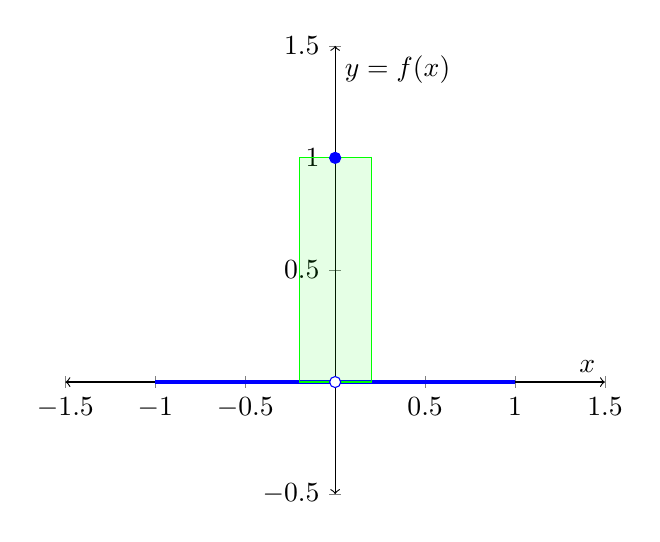
\begin{tikzpicture}
        \begin{axis}[
                xmin=-1.5,xmax=1.5,
                ymin=-0.5,ymax=1.5,
                axis x line=middle,
                axis y line=middle,
                axis line style=<->,
                xlabel={$x$},
                ylabel={$y=f(x)$},
            ]
            \addplot[blue, very thick, domain=-1:1]{0};
            \addplot[blue, soldot] coordinates{(0,1)};
            \addplot[blue, holdot] coordinates{(0,0)};
            \draw[green, fill=green, fill opacity=0.1] (-0.2,0) rectangle (0.2,1);
        \end{axis}
    \end{tikzpicture}
\end{center}
The above diagram depicts the upper sum $L_P(f)$ for some partition $P$, in which the subinterval containing $x=0$ is represented using a green rectangle of arbitrary width. Because this subinterval contains $x=0$, for which $f(x)=1$, its height is this supremal value of 1. All other subintervals, therefore, have a height of zero, and are not included in this diagram. For this partition $P$, we have that the upper sum is simply the area of this rectangle
$$
    U_P(f)=(\text{area of the green rectangle})=1\cdot(\text{width})
$$
Depending on the chosen partition $P$, the width of the green rectangle can be as large or as small as desired; it can be as large as 2, the size of the domain of our integral, or arbitrarily small, but not zero. In other words, the set of all upper sums is simply the set of all areas for some width $0<w\leq 2$.
$$
    \{\text{upper sums}\}=\{1\cdot w:w\in(0,2]\}=(0,2]
$$
Furthermore, the \textit{upper integral}, the infimum of the set of all upper sums is
$$
    \overline{\int_{-1}^{1}}(f)=\inf\{\text{upper sums}\}=\inf(0,2]=0
$$
Therefore, we have that
$$
    \underline{\int_{-1}^{1}}(f)=\overline{\int_{-1}^{1}}(f)=0
$$
and that $f$ is integrable on $[-1,1]$, and $\displaystyle\int_{-1}^1 f(x)dx=0$.
\subsubsection{A Non-Integrable Function}
There are many non-integrable functions, one of the most well known of which is called the Dirichlet function.
$$
    f(x)=\begin{cases}1&\text{if $x\in\Q$}\\0&\text{if $x\notin\Q$}\end{cases}
$$
In other words, $f(x)$ is $1$ if $x$ is a rational number, otherwise, $f(x)=0$. Let us consider the integral of this function on the interval $[0,1]$. To see why this function is not integrable, consider the following theorem.
\begin{theorem}[``Rational Number Theorem'']
    On every interval $[a,b]$ (where $a,b\in\R$ and $a<b$),
    \begin{itemize}
        \item There exists some $x\in[a,b]$ such that $x$ is a rational number ($x\in \Q$)
        \item There exists some $x\in[a,b]$ such that $x$ is an irrational number ($x\notin \Q$)
    \end{itemize}
    In other words, every interval $[a,b]$ contains both rational and irrational numbers.
\end{theorem}
A simple proof for this theorem can be found in the Appendix.\emptyline
Let $P=\{x_0,x_1,x_2,\dots,x_n\}$ be \textit{any} partition of $[0,1]$. For every subinterval $I=[x_{i-1},x_i]$, we have
\begin{itemize}
    \item $m_i=\displaystyle\inf_{x\in[x_{i-1},x_i]}f(x)=0$
    \item $M_i=\displaystyle\sup_{x\in[x_{i-1},x_i]}f(x)=1$
\end{itemize}
The reason for this is that every interval will have both rational and irrational numbers. Therefore, picking any subinterval and evaluating it on the function $f$ will yield a set $S$ for which at least one element is 0 and at least element is 1. Therefore, $\sup S=1$ and $\inf S=0$. As a result, our upper sum (again, for any partition $P$), will consist of only rectangles with height $M_i=1$, the widths of which add up to 1. Thus, we have
$$
    U_P(f)=1\cdot 1=1
$$
Similarly, we also have
$$
    L_P(f)=1\cdot 0=0
$$
Finally, we have
$$
    \overline{\int_{0}^{1}}(f)=\inf\{1\}=1
$$
and
$$
    \underline{\int_{0}^{1}}(f)=\sup\{0\}=0
$$
As we can see, the upper and lower sums are not equal, and thus, $f(x)$ is not integrable on the domain $[0,1]$. It is worth noting that the Dirichlet function \textit{is} integrable using the Lebesgue definition of integral; however, that is outside the scope of this course.
\subsection{Integrals as Limits}
\subsubsection{Introduction}
As stated before in the previous section regarding, \textit{finer} partitions produce lower upper sums and higher lower sums. Because the upper integral is the infimum of all possible upper sums, in a sense, the upper integral is the upper sum for ``the finest'' partition. Similarly, the lower integral is the lower sum for ``the finest'' partition. From this, it follows that if we were to have a limit as ``fineness approaches infinity'', we would be able to define integrals using limits.
\subsubsection{Definitions}
Recall the definition of \textit{fine} partitions.
\begin{definition}[Fine Partitions]
    Let $P$ and $Q$ be partitions of the interval $[a,b]$. \\
    We say $Q$ is \textbf{finer than} $P$ when $P\subseteq Q$.
\end{definition}
\begin{definition}[Norm of a Partition]
    Let $P=\{x_0,x_1,x_2,\dots,x_n\}$ be a partition of $[a,b]$. \\
    For each $i=1,2,\dots, n$, let $\Delta x_i=x_i-x_{i-1}$. \\
    The \textbf{norm} of $P$ is
    $$
        \norm{P}=\max\{\Delta x_1,\Delta x_2,\dots,\Delta x_n\}
    $$
\end{definition}
\subsubsection{Integrals as Limits}
From the above two definitions, we have the following theorem:
\begin{theorem}
    Let $f$ be a bounded function on $[a,b]$.
    $$
        \underline{\int_a^b}(f)=\lim_{\norm{P}\to 0} L_P(f)
    $$
    and
    $$
        \overline{\int_a^b}(f)=\lim_{\norm{P}\to 0} U_P(f)
    $$
\end{theorem}
What this theorem states is that
$$
    \forall \varepsilon>0,~\exists \delta>0~~\text{such that}~~\forall\text{partition $P$ of $[a,b]$},~\norm{P}<\delta\implies \left|\underline{\int_a^b}(f)-L_P(f)\right|<\varepsilon
$$
In other words, as the norm of a partition $P$ approaches zero, the difference between its lower sum and the actual lower integral also approaches zero.
\emptyline
Because this theorem involves the domain of all possible partitions for a given interval $[a,b]$, it does not simplify computation. By defining a specific way in which the norm of our partitions approaches zero, we simplify this definition.
\begin{theorem}
    Pick a sequence of partitions $P_1,P_2,P_3,\dots$ for the interval $[a,b]$ satisfying
    $$
        \lim_{n\to\infty}\norm{P_n}=0
    $$
    Then,
    $$
        \underline{\int_a^b}(f)=\lim_{n\to\infty}L_{P_n}(f)
    $$
    and
    $$
        \overline{\int_a^b}(f)=\lim_{n\to\infty}U_{P_n}(f)
    $$
    \hr
    The simplest example of such a sequence is the sequence that breaks the interval $[a,b]$ into $n$ equally sized subintervals:
    $$
        P_n=\left\{a+\frac{t(b-a)}{n}:t\in\{0,1,2,\dots,n\}\right\}
    $$
\end{theorem}
This definition of integral using limits is more useful than the previous one, since it takes the more intuitive concept of some number approaching infinity, rather than the norm of a partition approaching zero across the domain of all partitions.
\subsection{Riemann Sums}
\subsubsection{Definition}
\begin{definition}
    Let $f$ be a bounded function on the interval $[a,b]$. \\
    Let $P=\{x_0,x_1,x_2,\dots,x_n\}$ be a partition of $[a,b]$. \\
    For each $i=1,2,\dots,n$:
    \begin{itemize}
        \item Let $\Delta x_i=x_i-x_{i-1}$
        \item Choose a number $x_i^*\in[x_{i-1},x_i]$ (for simplicity, we can take $x_i^*=x_{i-1}$ or $x_i^*=x_i$)
    \end{itemize}
    Then
    $$
        S_P^*(f)=\sum_{i=1}^nf(x_i^*)\cdot\Delta x_i
    $$
    is called a \textbf{Riemann sum} for $f$ and $P$.
\end{definition}
Notice that we say \textit{a} Riemann sum rather than \textit{the} Riemann sum. Because we arbitrarily choose $x_i^*$, there are infinitely many Riemann sums. One common choice is to take $x_i^*=x_{i-1}$. This is called a \textit{left Riemann sum}, because it uses the left-hand value of each subinterval. To denote this choice of $x_i^*$, we denote the Riemann sum $S_P^*$.
\subsubsection{Riemann Integrals}
The relationship between Riemann sums and integrals can be summarized in the following theorem:
\begin{theorem}
    Let $f$ be a bounded function on the interval $[a,b]$. Assume $f$ is integrable on $[a,b]$.
    \begin{itemize}
        \item Pick a sequence of partitions $P_1,P_2,P_3,\dots$ for the interval $[a,b]$ satisfying
        $$
            \lim_{n\to\infty}\norm{P_n}=0
        $$
        \item On each subinterval of each partition, pick $x_i^*\in[x_{i-1},x_i]$. \\
    \end{itemize}
    Then
    $$
        \int_a^b f(x)dx=\lim_{n\to\infty} S_{P_n}^*(f)
    $$
    \hr
    \begin{itemize}
        \item The simplest example of such a sequence is the sequence that breaks the interval $[a,b]$ into $n$ equally sized subintervals:
        $$
            P_n=\left\{a+\frac{t(b-a)}{n}:t\in\{0,1,2,\dots,n\}\right\}
        $$
        \item The simplest choice of $x_i^*$ would be $x_i^*=x_i$
    \end{itemize}
\end{theorem}
Sometimes, this theorem is represented using the single formula:
$$
    \textcolor{blue}{\int_a^b} f(x)\textcolor{red}{dx}=\lim_{n\to\infty}\left[\sum_{i=1}^n f(x_i^*)\cdot\textcolor{red}{\Delta x_i}\right]
$$
\section{Unit 8: The Fundamental Theorem of Calculus}
\section{Appendix}
\subsection{Proof of the ``Rational Number Theorem''}
\begin{proof}
    Let $a,b\in\R$ such that $a<b$. \\
    Consider a natural number $n$ such that
    $$
        \frac{\sqrt 2}{n}<b-a
    $$
    (Such a number can be found by taking $\ceil*{\frac{\sqrt 2}{b-a}}$). \\
    Let $w=\frac{\sqrt{2}}{n}$. Notice that $w$ is an irrational number, since $\sqrt{2}$ is irrational. Additionally, $w+a$ is irrational. We also have $a<a+w<b$, since $w<b-a$. Thus, $w+a\notin\Q$ and $w+a\in[a,b]$. To instead find a \textit{rational} number, take $\frac{1}{n}$ instead of $\frac{\sqrt{2}}{n}$.
\end{proof}
\end{document}
